\section{Evaluation}
This section first introduces the datasets we used for 
the evaluation and then present four experiments. The first experiments
compare the performance of three models specifically targeting
data imbalance on Huangpu district. The second experiment examines
the effectiveness of our features by comparing the accuracy of our
primary model (decision tree + SMOTE) with some of the features
turned off. The third experiment evaluates the same area traffic
predication by comparing our model with two baselines: Baidu map
prediction and a simple time series model. The last experiment
evaluates the cross area prediction by training on the data from one
Shanghai district and testing on another.

\subsection{Datasets}
%After training the training set using LIBLINEAR, we obtained the model which could be used to test the scores on the test set, by comparing the predicted labels with the correct labels. We are able to easily predict a test set by using the \texttt{predict} program, also provided by LIBLINEAR. Note that the test data set are also being scaled with the same scaling parameter as the training set, that is, the test data is on the same data scale and range with the testing data on each feature. 
Our training and test data are the map features and live traffic data 
of four districts of Shanghai, China: Huangpu (HP), Changning (CN), 
Baoshan (BS) and Minhang (MH), extracted from Baidu Map. 
The first two districts are smaller but populous downtown districts 
with more business and commercial
destinations; the rest are suburban districts with larger area and 
contain more industrial and residential locations. 

In this work, we consolidate Baidu's POI classification into
a total of 37 types, and use bounded POI search API to query
all the POIs of all types, both on level 1 and level 2,
in a recursive manner: first query the entire district,
and if the number of returned results is equal to the API's maximum limit,
the bounding box is splitted into four equal sub-areas, with
small overlaps between them, until the number of returned POIs is less
than the limit. \tabref{tbl:poistats} shows the number of Baidu Map's 
POIs of some types in four evaluation areas. As Minhang and Baoshan 
district are larger than Huangpu and Changning district, the 
total numbers of POIs are higher in those areas. As a urban center district, 
Huangpu is having large amount of shopping places considering the area. 
Also, as being more suburban district and where more 
industries gather, there are significantly more factories 
in these district. It is shown that our selection of the 
datasets is sufficiently diverse and interesting.

\begin{table}[th]
	\centering
	\caption{An overview statistics of POI data}
	\label{tbl:poistats}
	\begin{tabular}{|c|c|c|c|c|}
		\hline
		& HP & CN & MH & BS \\ \hline \hline
		Residential & 13173   & 14451     & 17884   & 20559   \\ \hline
		Business    & 12965   & 11465     & 21753   & 13716   \\ \hline
		Shopping    & 7959    & 4734      & 11574   & 7103    \\ \hline
		Factory     & 44      & 44        & 565     & 671     \\ \hline
		Other       & 16718   & 15006     & 30699   & 20399   \\ \hline
		Total       & 50859   & 45700     & 82475   & 62448   \\ \hline
	\end{tabular}
\end{table}

The traffic information as well as other non-geospatial features such as weather and rental prices were crawled from May 19 to May 25 and from May 28 to June 1, 2016. The first 7 days of data is used for training while
the remaining 5 days are used for testing.

Our dataset is intrinsically imbalanced. \tabref{tab:imbal} shows the 
class distribution in the ground truth data of all four districts.

\begin{table}[th]
\centering
\caption{Imbalanced distribution of classes}
\label{tab:imbal}
\begin{tabular}{|c|c|c|c|c|} \hline
 & Green & Yellow & Red & Deep Red \\ \hline
Support & 3,481,345 & 174,106 & 41,912 & 3808 \\ \hline
\end{tabular}
\end{table}

Due to the imbalance nature of this data, our primary metric of
evaluation is the F1-score for each class label, rather than
overall accuracy for predicting all the road segments.
 
%so that compared to the training set, the test set is the future time data, which could correctly and scientifically measure and test our model's performance. In our case, the values' ranges between features vary largely due to the different type and aspect of the feature extraction and data source, and such scaling will help with the accuracy.
%
%As stated in the previous section, our problem is mainly dealing with telling rare classes that happens from one very large class. Classification and evaluation such imbalanced classes are real challenges, because accuracy no longer representing the model's correctness effectively, thus the optimization of parameter in common algorithms are not reliable anymore using accuracy as metric.
%
%In order to assess the model trained, we would introduce three scoring and evaluation methods use: Precision, Recall and F1 metrics.
%
%Precision-Recall metric are usually used to evaluate classifier output quality. In information retrieval, precision is a measure of result relevancy, while recall is a measure of how many truly relevant results are returned. A high area under the curve represents both high recall and high precision, where high precision relates to a low false positive rate, and high recall relates to a low false negative rate. High scores for both show that the classifier is returning accurate results (high precision), and returning a majority of all positive results (high recall).
%
%A system with high recall but low precision returns many results, but most of its predicted labels are incorrect when compared to the training labels. A system with high precision but low recall is just the opposite, returning very few results, but most of its predicted labels are correct when compared to the training labels. An ideal system with high precision and high recall will return many results, with all results labeled correctly.
%
%Precision ($ P $) is defined as the number of true positives ($ T_p $) over the number of true positives plus the number of false positives ($ F_p $).
%\begin{align}
%P = \frac{T_p}{T_p+F_p}
%\end{align}
%Recall ($ R $) is defined as the number of true positives ($ T_p $) over the number of true positives plus the number of false negatives ($ F_n $).
%\begin{align}
%R = \frac{T_p}{T_p + F_n}
%\end{align}
%These quantities are also related to the ($ F_1 $) score, which is defined as the harmonic mean of precision and recall.
%\begin{align}
%F1 = 2\frac{P \times R}{P+R}
%\end{align}
%It is important to note that the precision may not decrease with recall. The definition of precision ($ \frac{T_p}{T_p + F_p} $) shows that lowering the threshold of a classifier may increase the denominator, by increasing the number of results returned. If the threshold was previously set too high, the new results may all be true positives, which will increase precision. If the previous threshold was about right or too low, further lowering the threshold will introduce false positives, decreasing precision.
%Recall is defined as $ \frac{T_p}{T_p+F_n} $, where $ T_p+F_n $ does not depend on the classifier threshold. This means that lowering the classifier threshold may increase recall, by increasing the number of true positive results. It is also possible that lowering the threshold may leave recall unchanged, while the precision fluctuates.
%

\subsection{Model Evaluation}

%Our first model is a linear multi-class SVM with weights. 
%Although it can have high accuracy in Green class, 
%this naive model still is far from satisfaction because of its 
%low F1-score in any other classes.
%The rebalance strategy here is random oversampling, which seems to be simple.
%One obvious advantage of this model over the other models tested is that 
%the training process is faster more efficient.
%Then we optimize this model by binary decision tree model where each node is a binary
%SVM trained from data rebalanced with SMOTE  or simply by SVM with miss-classification penalty.
%Our experiment results show that binary decision tree with weighted SVM perform the best.
%So we build our model by combining decision tree with weighted SVM.

We compare multi-class SVM model with weight (SVM+w) with two of 
our decision tree ensemble models, decision tree of weighted
SVM (DT+SVM+w) and decision tree with SMOTE (DT+SMOTE\cite{chawla2002smote})
for predicting traffic of Shanghai's 
Huangpu district. 
To illustrate the severity of data imbalance issue on classfication performance,
we also compare with the basic unweighted multi-class SVM (SVM) 
as another baseline. \tabref{tab:modelselect} shows the F1 for predicting
green, yellow, red and deep red classes. 

The shortcoming of DT+SVM+w is that it's cost of error can be too high, 
which means that if one classifier makes mistake, 
the prediction will be worse and worse because it has no recursive methods.  
And the reason why we didn't select SMOTE as a 
solution to data imbalance problem is that the typical SMOTE have no method 
to over-sampling multi-class dataset. 
What's more, the time cost of SMOTE are quite high than any other method. 
Actually, if we use SMOTE, one often apply SMOTE with ENN or 
Tomek Link \cite{Batista:2004:SBS:1007730.1007735} to under-sample 
so as to make the new dataset valid, but the time cost will be even higher.

SVM+w, on the other hand, can be trained much more efficiently, the prediction
F1-score, except for the yellow class, is always higher than all other models. 
Therefore, we eventually choose the SVM+w as our primary model 
for its outstanding performance on the F1-score for Deep Red class and 
its fast training process. 

\begin{table}[ht]
\centering
\caption{F1-scores for predicting Huangpu district}
\label{tab:modelselect}
\begin{tabular}{|c|c|c|c|c|} \hline
Model/Class & Green & Yellow & Red & Deep Red \\ \hline\hline
SVM & {\bf 0.9582} & 0.0065& 0.0000 & 0.0000 \\ \hline
SVM+w & 0.9367 & 0.1587  & {\bf 0.1191}  & {\bf 0.0049} \\ \hline 
DT+SVM+w & 0.7118  & 0.1829 & 0.0749 & 0.0036\\ \hline 
DT+SMOTE & 0.7982 & {\bf 0.1969} & 0.0820 & 0.0042\\ \hline 
\end{tabular}
\end{table}

\subsection{Feature Assessment}
To illustrate the effectiveness of our features, we train four models with each of the four types of our features(road density, local POI distribution, global routing features and rental price). And then we  individually turn off one of them, and see the change in F1-score of the 4 classes.The results are shown in \figref{fig:4colorF1}, in which we can obviously conclude that every types of our feature are effective, especially POIs. 


The reason why POIs is a very important feature to describe the traffic situation is that it represents the popularity of certain road segments. Apart from that, we can find that other local features are also very helpful in training prediction models, for the fact that local features like \texttt{roadType} and \texttt{roadDensity} are very good indicators of traffic status.


\begin{figure*}[th]
\centering
\begin{subfigure}[t]{0.495\columnwidth}
	\resizebox{1.05\columnwidth}{!}{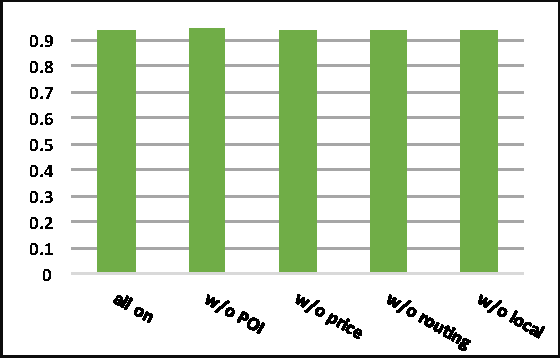
\includegraphics{figures/eval/Green.pdf}}
\end{subfigure}
\hfill
\begin{subfigure}[t]{0.495\columnwidth}
	\resizebox{1.05\columnwidth}{!}{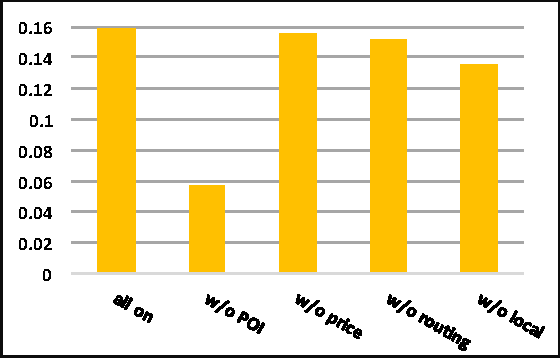
\includegraphics{figures/eval/Yellow.pdf}}
\end{subfigure}
\hfill
\begin{subfigure}[t]{0.495\columnwidth}
	\resizebox{1.05\columnwidth}{!}{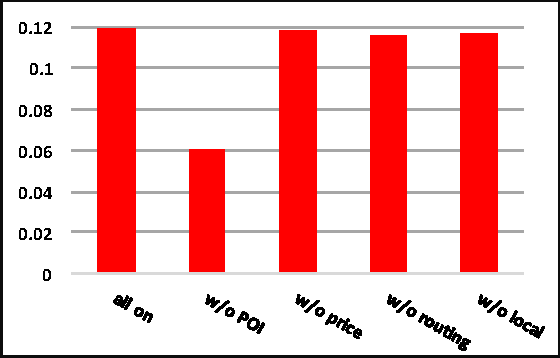
\includegraphics{figures/eval/Red.pdf}}
\end{subfigure}
\hfill
\begin{subfigure}[t]{0.495\columnwidth}
	\resizebox{1.05\columnwidth}{!}{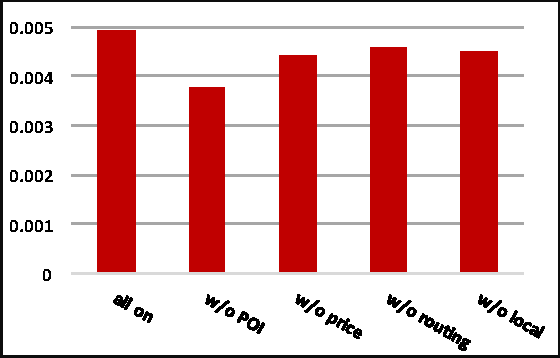
\includegraphics{figures/eval/DeepRed.pdf}}
\end{subfigure}

\caption{F1-score with some features turned off for
traffic conditions green, yellow, red and deep red}
\label{fig:4colorF1}
\end{figure*}


\subsection{Same-area Prediction}

In fact, Baidu Map also has a traffic prediction system as well, however, it predicts traffic for an area only
after Baidu has enough amount of historical data for the area. We sampled the Baidu's prediction at a historical time point (at one-hour interval) and use this as a kind of baseline.

Using the Huangpu district as an example, we first show the 
effect of date and time on the average prediction accuracy over 
5 days for all methods. 

Accuracy is defined as percentage of road segments that is correctly predicted. 
\figref{fig:daytimeacc} shows the accuracy results which compares our 
weighted SVM model with the Baidu Map's system. We can see that prediction accuracy at rush hours (9:00 and 17:00) is 
generally lower than other times of the day in both two results. This is because rush hour traffic is more volatile and 
exceptional events such as accidents may happen at different locations, 
which makes it hard to predict.

As a result, we reached an accuracy of 87.425\% while Baidu Map has an accuracy of 82.798\%. 


In Table~\ref{tbl:baiduf1}, we could see another evaluation result of our model compared Baidu's system. Although the F1-score of our system is a little bit lower than Baidu's, but our recall value is quite higher than Baidu's. Considering the application of the traffic prediction system, the recall value is a more important indicator, because it's not a very bad situation when we told a person that a road is slow but actually it is not that slow. But it can cause severe problems when we told someone a certain road is fast, but actually the road is actually very slow. Thus, our system is more applicable in real-world.

%The count of data instances are aggregated into time periods. 
%Readers may note that the total number of data instances of Baidu Map traffic prediction is always larger than ours, it is because that though both of them covered the whole Huangpu District, the points sampled for our test data is a bit smaller than the points sampled by Baidu Map, where the points were selected in a rectangular bounding box, which consists of some marginal data outside Huangpu District.

%explain and argue

There's some differences between the basic approach of our system and Baidu's
prediction system. We mainly consider the affects of both the global and local geospatial 
surroundings on traffic, while Baidu Map uses mainly temporal 
historical data at the location to make prediction. Additionally, Baidu is the only true owner of the original consecutive data so that it can treat this issue as a regression problem of the average of the speed. On the contrary, we can only get the result of its classification. Thus, we lost lots of meaningful data and therefore Baidu's prediction result are not an exactly fair comparison.
%And Table \ref{tbl:hamresult} shows the precision, recall and F1-score of the whole prediction of HAM.

\begin{figure}[th]
\centering
\resizebox{0.8\columnwidth}{!}{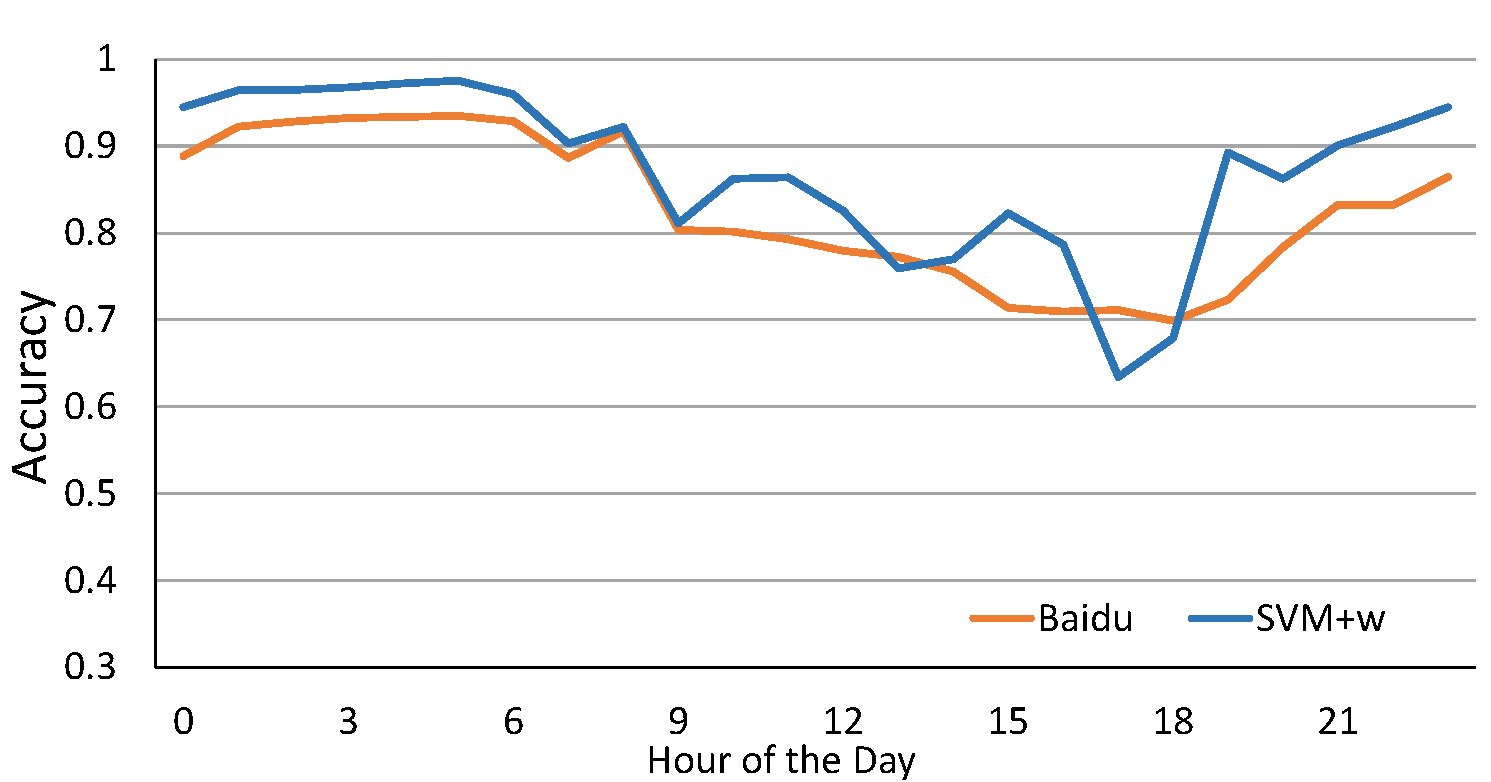
\includegraphics{figures/eval/accuracywithbaidu.pdf}}
\caption{Prediction accuracy in a day for Huangpu District}
\label{fig:daytimeacc}
\end{figure}


%\figref{fig:4distf1} shows the average F1-scores of all methods for predicting
%green, yellow, red and deep red conditions respectively, on four different
%districts. 
%\KZ{Discuss some more here..}

\begin{table}[]
	\centering
	\caption{Comparison of scores on red and deep red class of Baidu Map prediction with our system}
	\label{tbl:baiduf1}
	\begin{tabular}{|c|c|r|r|c|r|r|}
		\hline
		\multirow{2}{*}{} & \multicolumn{3}{c|}{Baidu Map}                                                            & \multicolumn{3}{c|}{Our System}                                                           \\ \cline{2-7} 
		& P                   & \multicolumn{1}{c|}{R} & \multicolumn{1}{c|}{F1} & P                   & \multicolumn{1}{c|}{R} & \multicolumn{1}{c|}{F1} \\ \hline
		Red               & \multicolumn{1}{r|}{0.255} & 0.110                      & 0.154                        & \multicolumn{1}{r|}{0.096} & 0.157                      & 0.119                        \\ \hline
		Deep Red          & \multicolumn{1}{r|}{0.000}      & 0.000                           & 0.000                             & \multicolumn{1}{r|}{0.003} & 0.233                      & 0.005                        \\ \hline
	\end{tabular}
\end{table}


%\begin{figure}[th]
%	\centering
%	\resizebox{\columnwidth}{!}{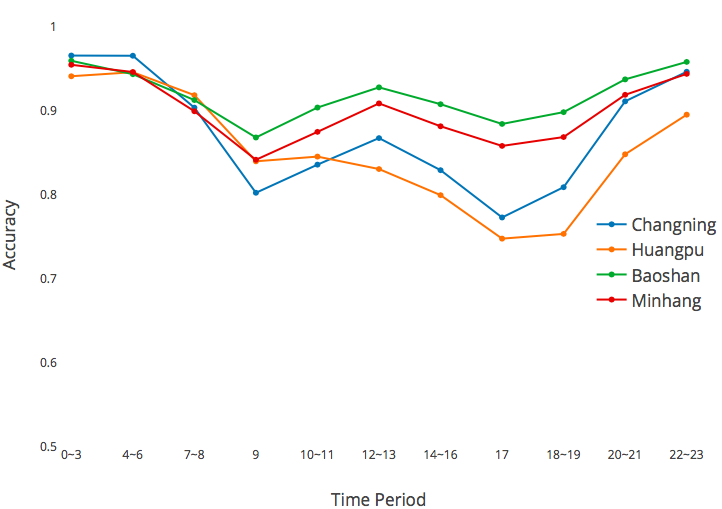
\includegraphics{figures/results/baidu.png}}
%	\caption{Accuracy of Baidu Prediction on different time periods. }
%	\label{fig:baidures}
%\end{figure}
%
%\begin{figure}[th]
%	\centering
%	\resizebox{\columnwidth}{!}{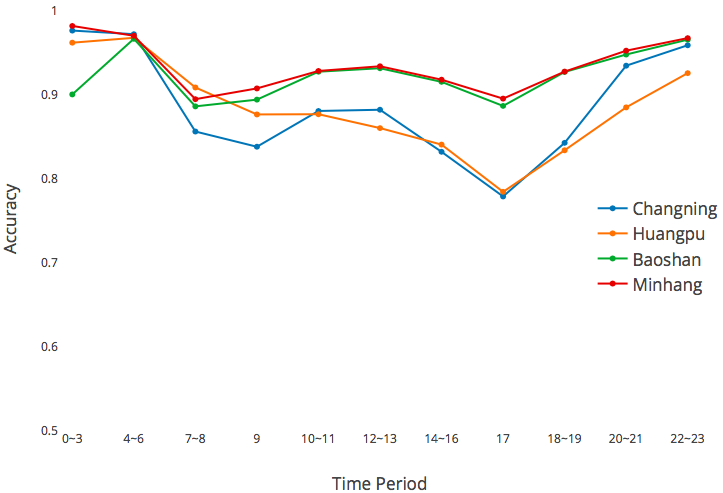
\includegraphics{figures/results/ham.png}}
%	\caption{Accuracy of HAM Prediction on different time periods. }
%	\label{fig:hamres}
%\end{figure}
%
%
%
%
%%Baidu Res
%\begin{table}[th]
%	\centering
%	\caption{Precision, recall and F1 scores of Baidu's result}
%	\label{tbl:baiduresult}
%	\begin{tabular}{l|l|l|l|l}
%		\hline
%		Class                          & Precision & Recall & F1 Score & Support \\ \hline
%		Green (Good)                   & 0.96      & 0.94   & 0.95     & 3260235  \\ \hline
%		Yellow (Slow)                  & 0.23      & 0.37   & 0.28     & 63564   \\ \hline
%		Red (Congested)                & 0.21      & 0.11   & 0.15     & 4744    \\ \hline
%		Deep Red (Heavy) & 0.01      & 0.03   & 0.02     & 144     \\ \hline
%		Avg / Total                    & 0.89      & 0.89   & 0.89     & 3328687  \\ \hline
%	\end{tabular}
%\end{table}
%
%
%%HAM Res
%\begin{table}[th]
%	\centering
%	\caption{Precision, recall and F1 scores of HAM's result}
%	\label{tbl:hamresult}
%	\begin{tabular}{l|l|l|l|l}
%		\hline
%		Class                          & Precision & Recall & F1 Score & Support \\ \hline
%		Green (Good)                   & 0.96      & 0.96   & 0.96     & 4607752  \\ \hline
%		Yellow (Slow)                  & 0.28      & 0.26   & 0.27     & 53060   \\ \hline
%		Red (Congested)                & 0.27      & 0.09   & 0.13     & 3973    \\ \hline
%		Deep Red (Heavy) & 0.003      & 0.01   & 0.01     & 123     \\ \hline
%		Avg / Total                    & 0.93      & 0.93   & 0.93     & 4664878  \\ \hline
%	\end{tabular}
%\end{table}
%
%\begin{table}[th]
%	\centering
%	\caption{Precision, recall and F1 scores of our model's result}
%	\label{tbl:testresult}
%	\begin{tabular}{l|l|l|l|l}
%		\hline
%		Class                          & Precision & Recall & F1 Score & Support \\ \hline
%		Green (Good)                   & 0.93      & 0.93   & 0.93     & 716106  \\ \hline
%		Yellow (Slow)                  & 0.24      & 0.10   & 0.14     & 53039   \\ \hline
%		Red (Congested)                & 0.07      & 0.14   & 0.09     & 9400    \\ \hline
%		Deep Red (Heavy) & 0.00      & 0.24   & 0.01     & 215     \\ \hline
%		Avg / Total                    & 0.87      & 0.87   & 0.87     & 778760  \\ \hline
%	\end{tabular}
%\end{table}
%


%See Table~\ref{tbl:testresult} for the scores of three different performance metrics the test result with popular way features representing the non-local geospatial features introduced in Section~\ref{sec:nonlocalfeatures}, and also with correct and identical data set scaling. From the scores of result data, we can see how big the impact of data imbalance issue can be. As seen in the table, the overall scores for predicting traffic that is good, which is the most popular class, is really out performing those for other minor classes, which is as high as 0.93. The scoring metrics are taking the distribution into consideration, and we can see that our system predict poorly for heavy traffic situations, especially the red and deep red ones. It is seen here that while doing cross-validation can help optimize our model, the imbalance issue would also break the evaluation. For imbalanced datasets, accuracy may not be a good criterion for evaluating a model. It may be better to conduct cross-validation and prediction with respect to different criteria (F1-score, AUC, etc.). We achieved this model by feature engineering worked by trying and testing with our without the set of feature, and compare various metrics, not limited to just accuracy, to make feature selection and achieve near optimal model. The tables also show that normalization and regularization of data set is crucial for linear SVC, which is sensitive to varying ranges. Besides, getting the scaling parameter right and consistent are crucial in such an application with large varying feature value ranges.
%
%
%

%Besides from the relatively close and good prediction rate during non-rush hours or weekdays, we perform sometimes better at rush hours where traffic anomalies appears more often. It is seen that most of the time our test result using mere linear SVC model exceeds the Baidu Map's traffic prediction result and accuracy based on time-series historical data, which is a great evidence that feature engineering on both local and non-local geospatial data indeed contribute to the model. It is also seen that at rush hours on workdays, the prediction accuracy is significantly lowered due to the model not performing so well while classifying extremely small classes, which is heavy traffic jam. Also, one should also notice that there are some test time periods that our system perform much worse than the Baidu Map traffic prediction, like the accuracy at 17 pm, May 31 is as low as 65.327\%, while the accuracy of Baidu Map at this time is 70.620\%, and like the accuracy at 20-23 pm, May 31 is also showing a large accuracy drop-down as Baidu Map's is 82.841\% and ours is 70.925\%. It is apparently anomalies in our data set, since the trend of accuracy simply changed a lot at this time, compared with the accuracy at the other days at the same time. We still need to investigate more on this issue, and looking deep into the prediction data, we found that our model performs really bad while having lots of traffic jams happening in the area which is generally low in probability. We still need to collect more and more data, since currently we only used 7 days of traffic data, which is far from enough for the model to be performing well against such anomalies when sudden outliers or events like holiday, extreme weather or traffic accident happens. That means our current model is sensitive and not robust enough.

%\begin{table*}[th]
%	\centering
%	\caption{The prediction result evaluation of our model compared to the traffic prediction data collected from Baidu Map, and all testing and comparison were done within the area of Huangpu District, Shanghai, and test set divided and predicted on hourly basis.}
%	\label{tbl:resultcomparison}
%	\begin{tabular}{|c|c|c|c|c|c|c|c|}
%		\hline
%		\multirow{2}{*}{Date} & \multirow{2}{*}{Hour} & \multicolumn{3}{c|}{Baidu Map Traffic Prediction} & \multicolumn{3}{c|}{Our Test Result} \\ \cline{3-8} 
%		&                       & \#Correct      & \#All        & Accuracy(\%)     & \#Correct  & \#All   & Accuracy (\%) \\ \hline
%		\multirow{3}{*}{5.28} & 16-17                 & 38465          & 52393        & 73.416            & 18366      & 24330   & 75.487        \\ \cline{2-8} 
%		& 18                    & 24730          & 34920        & 70.819            & 12688      & 16211   & 78.268        \\ \cline{2-8} 
%		& 19-23                 & 54783          & 69869        & 78.408            & 24336      & 32449   & 74.998        \\ \hline
%		\multirow{5}{*}{5.29} & 0-8                   & 193174         & 208941       & 92.454            & 93692      & 97396   & 96.197        \\ \cline{2-8} 
%		& 9-11                  & 72256          & 87335        & 82.734            & 35445      & 40540   & 87.432        \\ \cline{2-8} 
%		& 12-17                 & 61488          & 87323        & 70.414            & 34914      & 40545   & 86.112        \\ \cline{2-8} 
%		& 18-19                 & 38158          & 52407        & 72.811            & 21820      & 24344   & 89.632        \\ \cline{2-8} 
%		& 21-23                 & 73472          & 87338        & 84.124            & 37061      & 40562   & 91.369        \\ \hline
%		\multirow{5}{*}{5.30} & 0-7                   & 143761         & 156830       & 91.667            & 69386      & 73051   & 94.983        \\ \cline{2-8} 
%		& 10-14                 & 82890          & 104798       & 79.095            & 39897      & 48659   & 81.993        \\ \cline{2-8} 
%		& 15-16                 & 38132          & 52398        & 72.774            & 19986      & 24316   & 82.193        \\ \cline{2-8} 
%		& 19                    & 11831          & 17462        & 67.753            & 6958       & 8111    & 85.785        \\ \cline{2-8} 
%		& 20-23                 & 89219          & 104812       & 85.123            & 41987      & 48677   & 86.256        \\ \hline
%		\multirow{6}{*}{5.31} & 0-7                   & 95963          & 104387       & 91.930            & 46137      & 48711   & 94.716        \\ \cline{2-8} 
%		& 9                     & 26245          & 34940        & 75.114            & 13422      & 16217   & 82.765        \\ \cline{2-8} 
%		& 10-14                 & 80915          & 104797       & 77.211            & 37976      & 48655   & 78.052        \\ \cline{2-8} 
%		& 17                    & 12333          & 17464        & 70.620            & 5300       & 8113    & 65.327        \\ \cline{2-8} 
%		& 18-19                 & 23927          & 34928        & 68.504            & 11710      & 16222   & 72.186        \\ \cline{2-8} 
%		& 20-23                 & 43418          & 52411        & 82.841            & 17259      & 24334   & 70.925        \\ \hline
%		\multirow{3}{*}{6.1}  & 0-7                   & 126991         & 139389       & 91.105            & 59625      & 64923   & 91.840        \\ \cline{2-8} 
%		& 9                     & 14564          & 17469        & 83.371            & 6919       & 8090    & 85.525        \\ \cline{2-8} 
%		& 10-13                 & 40160          & 52402        & 76.638            & 20665      & 24304   & 85.027        \\ \hline
%		\multicolumn{2}{|c|}{Overall}                 & 1386875        & 1675013      & 82.798            & 675549     & 778760  & 86.747        \\ \hline
%	\end{tabular}
%\end{table*}
%

\subsection{Cross-area Prediction}
In this experiment, we train our SVM model from training data of
four different districts and use them to test the other districts.
\tabref{tab:cross} documents the F1-score on four different traffic
classes. As a comparison, we also show the results of
same-district prediction as well. From the table, we could see that in most cases our model yield good prediction results on cross-region prediction. From the POI statistics we have discussed before, the four districts are distinct to some extent in terms of both area, population and main gathering industries. 

There are some interesting facts in it, e.g the cross-region prediction results for green class of Changning, Minhang and Baoshan district using the model trained in Huangpu district are even better than Huangpu district itself. The reason for this may be the fact that those more suburban areas are less congested overall and having smaller number of popular POIs. For the more congested traffic conditions, the prediction is still doing well, such as the Huangpu district prediction using the Changning district model. These two districts are both urban areas with relatively similar characteristics, and good result means that our model is having good generalization of both geographical properties. There are, however, some test sets that performed worse than average, we considered it normal since the model trained in one district with specific characteristic will be weaker at predicting for a different area. For example, Baoshan district is an industrial district. Similarly, Minhang has many factories too, and that explains why models trained from Baoshan can predict for Minhang with relatively high F1 score of 0.0721.

In summary, we considered our cross-region prediction to be effective at predicting other geographically or characteristically similar areas without historical traffic data.

\begin{table}[th]
\centering
\caption{F1-score of cross-area prediction for 4 classes. T:Test data, 
M:Training data}
\label{tab:cross}
\caption*{Green}
\begin{tabular}{|c||c|c|c|c|}
\hline
\diagbox{T}{M} & HP & CN & MH & BS \\ \hline
HP & 0.9367 & 0.8166 & 0.7029 & 0.6854 \\ \hline
CN & {\bf 0.9443} & 0.9454 & 0.8803 & 0.8017 \\ \hline
MH & {\bf 0.9763} & 0.9613 & 0.9691 & 0.9559 \\ \hline
BS & {\bf 0.9689} & 0.9529 & 0.9515 & 0.9662 \\
\hline
\end{tabular}%

\caption*{Yellow}
\begin{tabular}{|c||c|c|c|c|}
\hline
\diagbox{T}{M} & HP & CN & MH & BS \\ \hline
HP & 0.1587 & {\bf 0.1705} & 0.1124 & 0.1248 \\ \hline
CN & 0.0509 & 0.1841 & 0.0970 & 0.0825 \\ \hline
MH & 0.0007 & 0.0549 & 0.0798 & {\bf 0.0721} \\ \hline
BS & 0.0040 & 0.0530 & 0.0458 & 0.0876 \\
\hline
\end{tabular}%

\caption*{Red}
\begin{tabular}{|c||c|c|c|c|}
\hline
\diagbox{T}{M} & HP & CN & MH & BS \\ \hline
HP & 0.1191 & 0.0440 & 0.0301 & 0.0277 \\ \hline
CN & 0.0426 & 0.1096 & {\bf 0.0831} & 0.0429 \\ \hline
MH & 0.0100 & 0.0387 & 0.0841 & 0.0406 \\ 
	\hline
BS & 0.0217 & 0.0414 & 0.0581 & 0.1124 \\
\hline
\end{tabular}%

\caption*{Deep Red}
\begin{tabular}{|c||c|c|c|c|}
\hline
\diagbox{T}{M} & HP & CN & MH & BS \\ \hline
HP & 0.0049 & 0.0002 & 0.0011 & 0.0002 \\ \hline
CN & 0.0027 & 0.0287 & 0.0013 & 0.0015 \\ \hline
MH & 0.0000 & 0.0043 & 0.0241 & 0.0022 \\ 
	\hline
BS & 0.0000 & 0.0005 & 0.0290 & 0.1002 \\
\hline
\end{tabular}%

\end{table}
